\documentclass[../main.tex]{subfiles}

\graphicspath{{\subfix{../images/}}}

\begin{document}

\section{Task 3.4}

Create a cycle accurate communication model of a master and slave module that uses the Avalon Streaming Bus Interface (ST). Simulate that a master are transmitting data to a slave module as illustrated in Figure (\ref{fig:avalon}). The slave should store received data from the master in a text file. Include in the model a situation where the data sink signals $\text{ready} = \text{'0'}$. The simulated result should be presented in the GTK wave viewer, so a VCD trace file must be created. It should e possible to configure the channel, error and data size define in a separate header file.

\begin{figure}[h]
    \centering
    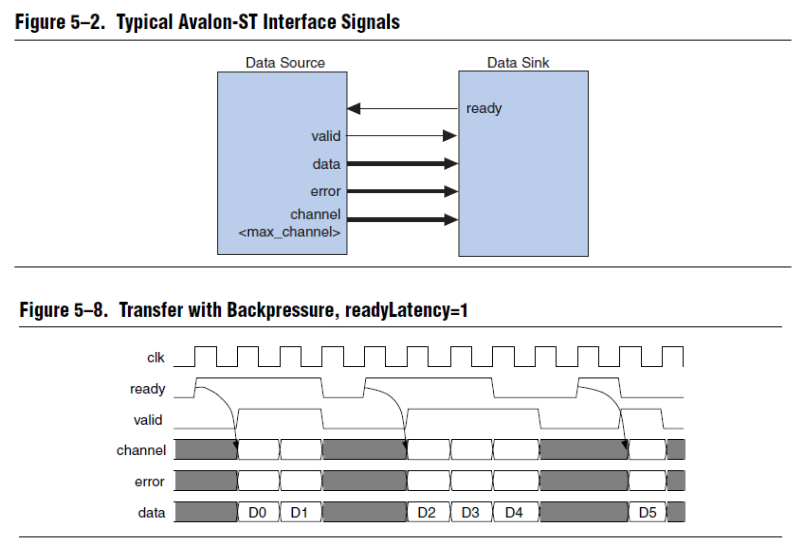
\includegraphics[width=0.9\textwidth]{task3_4.png}
    \caption{Avalon Streaming Bus Interface.}
    \label{fig:avalon}
\end{figure}

\subsection*{Solution}

\end{document}